\documentclass{article}
\usepackage{amsmath, amssymb, amsthm, amsfonts, bm}
\theoremstyle{remark}

\usepackage{physics}
\usepackage[a4paper, total={6in,10in}]{geometry}
\usepackage[dvipsnames]{xcolor}
\usepackage{xcolor-material}
\usepackage{hyperref}
    \hypersetup{colorlinks=true, linkcolor=ForestGreen}
\usepackage{graphicx}
    \graphicspath{{./img/}}
\usepackage{tikz}
\usepackage{ragged2e}

\usepackage{soul}
\usepackage{cancel}

\usepackage{booktabs}
\usepackage{cellspace}
\newcolumntype{L}[1]{>{\centering\arraybackslash}m{#1}}  % cell with auto-wrap, e.g. |L{0.2\linewidth}|L{0.8\linewidth}|
\usepackage{makecell}  % use Sc instead of c
\setlength{\cellspacetoplimit}{10pt}
\setlength{\cellspacebottomlimit}{10pt}

\newcommand{\where}[1]{\begin{flushright}where #1.\end{flushright}}
\newcommand{\wher}[1]{\begin{flushright}#1.\end{flushright}}
\newcommand{\mylabel}[2]{\hyperref[#1]{#2}\label{back:#1}}
\newcommand{\myref}[1]{\hyperref[back:#1]{$\bigstar$}\label{#1}}
\newcommand{\e}{\hat{\vb{e}}}  % unit vector
\newcommand{\s}[1]{\textsubscript{#1}}
\newcommand{\ppdv}[4][]{\left(\pdv[#1]{#2}{#3}\right)_{#4}}
\everymath{\displaystyle}
\begin{document}

\section*{Basic concepts}
\begin{enumerate}
    \item Extensive: proportional to $N$; Intensive: ratio of extensive
    \item $\dd U=T\dd S-p\dd V+\mu\dd N$
    \item Carnot's theorem $\frac{Q_1}{T_1}=\frac{Q_2}{T_2}$\newline
    \item Efficiency (for $T_2>T_1$)\begin{itemize}
        \item $\eta=\frac{\text{energy you care about}}{\text{work/heat you used}}$
        \item Carnot engine $\eta=\frac{\text{work done}}{\text{heat used}}=\frac{Q_2-Q_1}{Q_2}$
        \item Refrigerator $\eta=\frac{\text{heat removed}}{\text{work done}}=\frac{Q_1}{W}=\frac{Q_1}{Q_2-Q_1}$
        \item Heat pump $\eta=\frac{\text{heat you added}}{\text{work done}}=\frac{Q_2}{W}=\frac{Q_2}{Q_2-Q_1}\geq 1$
        \item $\eta=1-\frac{Q_1}{Q_2}$
    \end{itemize}
    \item $\dd S=\frac{\dd Q_{rev}}{T}\boxed{\geq\frac{\dd Q}{T}}$
    \item \fbox{Clausius' theorem $\oint\frac{\dd Q}{T}\leq 0$}
        \where{$\dd Q$ is heat rejected from engine}
        ($\dd Q_{irrev}<\dd Q_{rev}<0$ because friction means more heat released, making $\textstyle\oint\dd Q/T<0$)
    \item $C_V = \left(\dv{Q}{T}\right)_V = T\left(\pdv{S}{T}\right)_V = \left(\dv{U}{T}\right)_V$
    \item $C_p = \left(\dv{Q}{T}\right)_p = T\left(\pdv{S}{T}\right)_p = \left(\dv{H}{T}\right)_p$
    \item Latent heat $L=T(S_2-S_1)$
    \item Ideal gas \begin{align*}
        S &= C_V\ln T+nR\ln V+S_0(n)\\
          &= nc_V\ln T+nR\ln(V/n)+nS_0',
    \end{align*}\wher{$S_0(n)=nS_0'-nR\ln n$}
    \item \includegraphics*{Entropy_of_mixing.png}\newline
    $\Delta S = n_1 R\ln\left(\frac{V_1+V_2}{V_1}\right)+n_2 R\ln\left(\frac{V_1+V_2}{V_2}\right)$\begin{itemize}
        \item Gibbs' paradox: what if two gases are the same
        \item In the above equation, \textbf{reversible} isothermal expansion is assumed
        \item No process- is reversible for \textbf{indistinguishable} particles/gases
    \end{itemize}
    \item \begin{tabular}{|c|c|c|c|}
        H & Enthalpy & U+pV & \textbf{isobaric} heat transfer\\
        F & Helmholtz free energy & U-TS & \textbf{isothermal} work done\\
        G & Gibbs energy & U+pV-TS & $\boxed{G=\mu N}$\\
        $\Phi_G$ & Grand potential & $U-TS-\mu N$ & $\boxed{\Phi_G=-pV}$\\
    \end{tabular}\mylabel{mu_and_G}{$\bigstar$}
    \item If irreversible (heat flow from resevior to body) and constant $p$, $T$, \newline
            $-\frac{\dd G}{T} = -\frac{\dd U-T\dd S}{T}= -\dd S_{\text{res}}-\dd S_{\text{sys}} = \dd S_{\text{total}}$
    \item Thermodynamics variables\newline
        \begin{minipage}{0.7\linewidth}
            \begin{align*}
                T  = \left(\pdv{U}{S}\right)_V &= \left(\pdv{H}{S}\right)_p\\
                p = -\left(\pdv{U}{V}\right)_S &= -\left(\pdv{F}{V}\right)_T\\
                V = \left(\pdv{H}{p}\right)_S &= \left(\pdv{G}{p}\right)_T\\
                S = -\left(\pdv{F}{T}\right)_V &= -\left(\pdv{G}{T}\right)_p
            \end{align*}
        \end{minipage}
        \begin{minipage}{0.3\linewidth}
            \includegraphics*[width=\linewidth]{Thermodynamic_square.png}
        \end{minipage}

        The thermodynamic square\newline
        \fbox{Good Physicist Have Studied Under Very Fine Teachers}\newline
        Left vars $p$ and $S$ negative sign\newline
        $\text{var}=\text{sign}\left(\pdv{\text{opposite potential}}{\text{opposite var}}\right)_{\text{other var beside potential}}$

        Maxwell's relations\newline
        \begin{minipage}{0.5\linewidth}
            \begin{itemize}
                \item Pick a potential, draw $\Rsh$ and $\Lsh$ around it
                \item $\boxed{\left(\pdv{\ 1}{\ 2}\right)_3}$ \newline
                    (2nd derivative of the potential picked)
                \item Add sign = $\text{sgn}(1)\text{sgn}(2)\text{sgn}(3)$
            \end{itemize}
            Or use $\boxed{\pdv{(T,S)}{(p,V)}=1}$ \begin{itemize}
                \item $\pdv{(T,S)}{(x,y)}=\pdv{(p,V)}{(x,y)}$
                \item $(x,y)$ can be $(T,p)$, $(T,V)$, $(p,S)$, $(S,V)$
                \item $\oint\dd U=0 =\oint T\dd S-p\dd V$
                \item $\iint_A\dd p\dd V=\iint_A\dd T\dd S$
                \item Also by Jacobian transformation $\iint_A\dd T\dd S=\iint_A\pdv{(T,S)}{(p,V)}\dd p\dd V$
            \end{itemize}
        \end{minipage}
        \begin{minipage}{0.5\linewidth}
            \includegraphics*[width=\linewidth]{maxwell_relation_mnemonic.png}\newline
            \begin{align*}
                \left(\pdv{T}{V}\right)_S=-\left(\pdv{p}{S}\right)_V\\
                \left(\pdv{T}{p}\right)_S=\left(\frac{V}{S}\right)_p\\
                \left(\pdv{S}{V}\right)_T=\left(\pdv{p}{T}\right)_V\\
                \left(\pdv{S}{p}\right)_T=-\left(\pdv{V}{T}\right)_p
            \end{align*}
        \end{minipage}

        (better derive it for non-$pV$ systems)
    \item Partial derivative rules\begin{itemize}
            \item $\dd f=\ppdv{f}{x}{y}+\ppdv{f}{y}{x}\dd y$
            \item Maxwell's relations
            \item $\ppdv{x}{z}{y}=1/\ppdv{z}{x}{y}$ \mylabel{reciprocity_relations}{$\bigstar$}
            \item $\ppdv{x}{y}{z}\ppdv{y}{z}{x}\ppdv{z}{x}{y}=-1$
            \item Measurable quantities $C_V=T\ppdv{S}{T}{V}$, $C_p=T\ppdv{S}{T}{p}$
            \item Identify a \emph{generalized susceptibility}\begin{itemize}
                \item \emph{isobaric expansivity} $\beta_p=\frac{1}{V}\ppdv{V}{T}{p}$
                \item \emph{adiabatic expansivity} $\beta_S=\frac{1}{V}\ppdv{V}{T}{S}$
                \item \emph{isothermal compressibility} $\kappa_T=-\frac{1}{V}\ppdv{V}{p}{T}$
                \item \emph{adiabatic compressibility} $\kappa_S=-\frac{1}{V}\ppdv{V}{p}{S}$ (minus sign to keep it $+ve$)
            \end{itemize}
            \item Reversible adiabatic expansion $\boxed{pV^\gamma=\text{constant}}$, $\gamma=C_p/C_V=\kappa_T/\kappa_S$
        \end{itemize}
    \item Some identities\begin{itemize}
            \item $C_p-C_V=\frac{TV\beta_p^2}{\kappa_T}$
            \item isothermal atmosphere $p=p_0e^{-\frac{m_rgh}{RT}}$
            \item constant $T$, $p$, $\dd S_{\text{total}}=-\frac{\dd G}{T}$
            \item Gibbs-Helmholtz equation $U=-T^2\left(\pdv{F/T}{T}\right)_V$, $H=-T^2\left(\pdv{G/T}{T}\right)_p$
            \item Joule's expansion (adiabatic/free gas expansion) $\ppdv{U}{V}{T}=0$ because $U=U(T)$
        \end{itemize}
    \item Elastic rod\begin{itemize}
        \item $\dd U=T\dd S+f\dd x$
        \item Cross sectional area $A$ assumed constant always
        \item \emph{Isothermal Young's modulus} $E_T=\frac{\sigma}{\epsilon}=\frac{L}{A}\ppdv{f}{x}{T}$
        \item \emph{Linear expansivity at constant tension} $\alpha_f=\frac{1}{L}\ppdv{x}{T}{f}$ ($>0$ for wire, $<0$ for rubber)
        \item $\dd F = -S\dd T+f\dd x$, maxwell: $\ppdv{S}{x}{T}=-\ppdv{f}{T}{x}=AE_T\alpha_f$
                $\ppdv{S}{V}{T}=E_T\alpha_f$ (if $\alpha_f>0$, stretching increases entropy, wire absorbs heat. vice versa for rubber)
    \end{itemize}
    \item Surface tension\begin{itemize}
        \item Surface energy $=u(T)\dd A$
        \item $\dd U=T\dd S+\gamma\dd A$, $\gamma$ is surface tension (or Helmholtz free energy per unit area at constant $T$)
        \item $u(T)=\ppdv{U}{A}{T}$, $\dd S=\ppdv{S}{T}{A}+\ppdv{S}{A}{T}$, $\dd U=T\ppdv{S}{T}{A}\dd T+T\ppdv{S}{A}{T}\dd A+\gamma\dd A=
                T\ppdv{S}{T}{A}\dd T+\left(\gamma-T\ppdv{\gamma}{T}{A}\right)\dd A$

            $\boxed{u(T)=\gamma-T\dv{\gamma}{T}}$ ($\gamma$ independent of $A$)
        \item Usually $\dv{\gamma}{T}<0$, $u(T)>\gamma$
        \item Laplace pressure of a bubble $\Delta p=p\s{inside}-p\s{outside}=\frac{2\gamma}{R}$ (\mylabel{laplace_pressure}{Proof})
    \end{itemize}
    \item Paramagnetism\begin{itemize}
            \item $\dd U=T\dd S-m\dd B$
            \item Curie's law $\chi\propto\frac{1}{T}$, $\ppdv{\chi}{T}{B}<0$
            \item Assume $\chi\ll 1$, $B=\mu_0(H+M)\approx\mu_0 H$, $\chi=\lim_{H\rightarrow0}\frac{M}{H}\approx\frac{\mu_0M}{B}$
            \item Total magnetisation $m=MV$
            \item Maxwell relation $\ppdv{S}{B}{T}=\ppdv{m}{T}{B}\approx\frac{VB}{\mu_0}\ppdv{\chi}{T}{B}$
            \item Adiabatic temperature change $\ppdv{T}{B}{S}=-\ppdv{S}{B}{T}\ppdv{T}{S}{B}=-\frac{TVB}{\mu_0C_B}\ppdv{\chi}{T}{B}>0$, where $C_B=T\ppdv{S}{T}{B}$ is the heat capacity at constant $B$
            \item In labs, material can be cooled to a few millikelvin by adiabatic demagnetization (reduce $B$)
        \end{itemize}
    \item Intuition in a picture\begin{center}
            \includegraphics*[width=0.3\linewidth]{intuition_4_situations.png}
        \end{center}
\end{enumerate}

\section*{Phase transitions}
\begin{enumerate}
    \item EoS of gas\begin{itemize}
            \item Boyle's law for ideal gas: $pV=A_0$ where $A_0 $ is a constant. Simple but wrong
            \item Virial expansion: $pV=A_0+A_1p+A_2p^2+\cdots=B_0+B_1/V+B_2/V^2+\cdots$, $A_i=A_i(T)$
            \item The \emph{Boyle temperature} $T_B$ is when $A_1(T_B)=0$
            \item Gas have similar properties if plotted in reduced variables
                \begin{center}
                    \includegraphics*[width=0.5\linewidth]{gas_reduced_variables.png}
                \end{center}
                (Noticable deviation for $\mathrm{H_2}$ and He due to quantum effects)
            \item Real world applications: use measured data of compressibility factor $Z=\frac{pV}{nRT}$\newline
                \begin{center}
                    \includegraphics*[width=0.5\linewidth]{compressibility factor.png}
                \end{center}
        \end{itemize}
    \item Van der Waals' equation\begin{itemize}
            \item $\left(p+a\frac{n^2}{V^2}\right)(V-nb)=nRT$ for $n$ moles of gas
            \item Attraction between molecules reduces potential energy by $a\rho=a\frac{n}{V}$ for each molecule and some $a$.
                $U=U_0-a\frac{n^2}{V}$, $p=\ppdv{U}{V}{T}=p_0+\frac{an^2}{V^2}$
            \item Curves at different $T$. Curve might have negative $\kappa_T$, which is unstable.
                Curve with point of inflexion is the \emph{critical isotherm} with its \emph{critical point}, at \emph{Critical temperature} $T_c$. (thick line with dot)
                \begin{center}
                    \includegraphics*[width=0.5\linewidth]{van_der_waal.png}
                \end{center}
                \begin{itemize}
                    \item Critical volume $V_c=3b$
                    \item $T_c=8a/27Rb$
                    \item $p_c=a/27b^2$
                    \item $\kappa_T=1/0$
                    \item Boyle temperature $T_B=a/Rb$ ($1/V$ expansion)
                    \item (Hint: $p=\frac{RT}{V-b}-\frac{a}{V^2}$, $\ppdv{p}{V}{T}=0$, $\ppdv[2]{p}{V}{T}$)
                \end{itemize}
            \item \begin{minipage}{0.4\linewidth}
                    \includegraphics*[width=\linewidth]{van_der_waal_G.png}
                \end{minipage}
                \begin{minipage}{0.6\linewidth}
                    \begin{itemize}
                        \item $p=-\ppdv{F}{V}{T}$
                        \item $F=f(T)-RT\ln(V-b)-\frac{a}{V}$
                        \item Constant $p$ and $T$, minimize $G=F+pV$
                        \item Equilibrium states minimizes $G$ ($\dd G=-T\dd S_{total}$, maximizes entropy)
                        \item Predicts \emph{metastable states} (BXYB) that only happens when not in equilibrium. AB liquid and BC gas \emph{coexist} at B.
                        \item BY supercooled gas, BX superheated liquid.
                    \end{itemize}
                \end{minipage}
            \item Find point B\begin{itemize}
                    \item Same Gibbs energy, $\int_{p_0}^{p_1}\ppdv{G}{p}{T}\dd p=0=\int_{p_0}^{p_1}V\dd p$ (The Maxwell construction)
                    \item \begin{center}
                            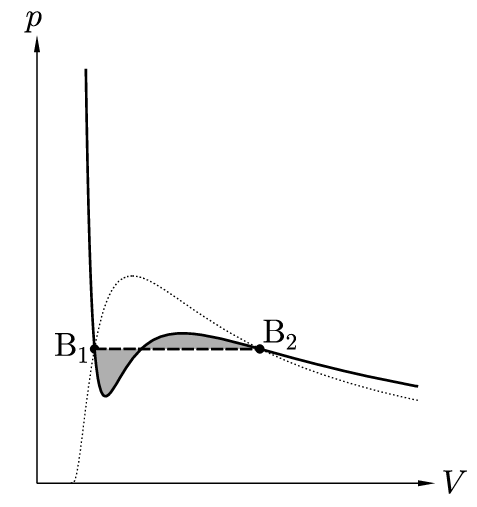
\includegraphics[width=0.5\linewidth]{van_der_waal_maxwell.png}
                        \end{center}
                    \item Usually goes straight from $B_1$ to $B_2$ at constant $p$ (approximation to a fast process I guess), unless liquid very pure and moves along the curve, then quickly moves across region of negative $\kappa_T$ to become gas
                    \item At point B and temperature $T_c$, the two states are indistinguishable. Also shown by other facts:
                        Densities at $T_c$ become identical, latent heat of vaporisation becomes 0.
                \end{itemize}
            \item Ways to cool van der Waals gas:\begin{itemize}
                    \item Joule expansion (freely expand)
                    \item Isothermal expansion
                    \item Joule-Kelvin expansion - high $p$ to low $p$, constant $H$. To see dropping pressure causes heating or cooling,
                        the \emph{inversion curve} is defined by $\mu_{JK}=0=T\ppdv{V}{T}{p}-V$ or $\ppdv{V}{T}{p}=\frac{V}{T}$; $\mu_{JK}=\ppdv{T}{p}{H}=-\frac{1}{C_p}\ppdv{H}{p}{T}$, $h_i=yh_L+(1-y)h_f$, $y=\frac{h_f-h_i}{h_f-h_L}$, the optimal pressure $p_i$ satisfies $\ppdv{y}{p_i}{T_i}=0$, or $\ppdv{h_i}{p_i}{T_i}=-C_p\mu_{JK}=0$, \underline{the best choice is $\mu_{JK}=0$ on the inversion curve}.
                \end{itemize}
        \end{itemize}
    \item Gibbs-Duhem equation $N\dd\mu=-S\dd T+V\dd p$\mylabel{gibbs_duhem}{$\bigstar$}
    \item Clausius-Clapeyron equation $\boxed{\dv{p}{T}=\frac{\Delta S}{\Delta V}=\frac{L}{T\Delta V}}$ \mylabel{cc_equ}{$\bigstar$}
    \item Phase change caveats\begin{itemize}
            \item Liquid/solid to gas $\Delta V=V\s{vap}-V\s{liq/solid}\approx V\s{vap}$
            \item Temperature dependence of latent heat usually ignored.\newline
                    For ideal gas, $L=L_0+(C_{p,\text{vapour}}-C_{p,\text{liquid}})T$
                    \mylabel{temp_dep_latent_heat}{$\bigstar$}
            \item Solid-liquid boundary, assume $\Delta V\ll1,L$ independent of $T$.\newline
                    $p=p_0+\frac{L}{\Delta V}\ln\left(\frac{T}{T_0}\right)$, $\left|\dv{p}{T}\right|\gg1$ (very steep)
            \item $\Delta V<0$ from ice to water, $\dv{p}{T}<0$
        \end{itemize}
\end{enumerate}

\section*{Statistical Intro}
\begin{enumerate}
    \item $\Omega=\Omega(E-E_i)\Omega(E-E_i)$
    \item $\beta=\dv{\ln\Omega}{E}$\newline
        (Condition for $T_1=T_2$ is $\dv{\Omega}{E_i}=0\implies\frac{\Omega(E_i)'}{\Omega(E_i)}=\frac{\Omega(E-E_i)'}{\Omega(E-E_i)}\implies\frac{\ln\Omega(E_i)}{E_i}=\frac{\ln\Omega(E-E_i)}{E_i}$)
    \item Boltzmann distribution $P(E_i)=\frac{e^{-\beta E_i}}{Z}$, partition function $Z=\sum_{j}e^{-\beta E_j}$, $\beta=\frac{1}{k_B T}$ \newline
        ($P(E_i)=\frac{\Omega(E-E_i)}{\Omega(E)})$
    \item Entropy $S=k_B\ln\Omega=\boxed{-k_B\sum_{i}p_i\ln p_i}$ \\ (intuition: Time averaged geometric mean/TAGM probability $p_{TAGM}=\sqrt[n]{\prod_i p_i^{np_i}}$, $np_i$ is number of microstates with probablility $p_i$ in time series of length $n$; Microstates multiply, entropies add, so take log)
    \item \includegraphics*[width=0.8\linewidth]{thermodynamic_variables__function.png}\newline
        ($U=\langle E\rangle$, $S=-k_B\sum_i P_i\ln P_i=\frac{U}{T}+k_B\ln Z$, $F=U-TS$)
    \item If $T$ is not too low (so energy gaps small, summation $\approx$ integral), and $T$ is not too high (modes are quadratic/harmonic)\begin{itemize}
            \item $\langle E\rangle =\int_{-\infty}^{\infty}EP(x)\dd x=\frac{\int_{-\infty}^{\infty}ax^2e^{-\beta ax^2}\dd x}{\int_{-\infty}^{\infty}e^{-\beta ax^2}\dd x}=\frac{1}{2\beta}=\frac{1}{2}k_B T$ (Feynmann's trick)
            \item If $E=\sum_{i=1}^na_ix_i^2$, \newline
                $\langle E\rangle=\int_{-\infty}^{\infty}\cdots\int_{-\infty}^{\infty} EP(x_1,\ldots,x_n)\dd x_1\cdots\dd x_n
                    \newline\null\ \quad=\sum_{i=1}^n\frac{\int_{-\infty}^{\infty}\cdots\int_{-\infty}^{\infty}a_ix_i^2e^{-\beta E}\dd x_1\cdots\dd x_n}{\int_{-\infty}^{\infty}\cdots\int_{-\infty}^{\infty}e^{-\beta E}\dd x_1\cdots\dd x_n}
                    \newline\null\ \quad=\sum_{i=1}^n\frac{\int_{-\infty}^\infty a_ix_i^2e^{-\beta a_ix_i^2}\dd x_i}{\int_{-\infty}^\infty e^{-\beta a_ix_i^2}\dd x_i}
                    =\sum_{i=1}^na_i\langle x_i^2\rangle=\sum_{i=1}^n\frac{k_BT}{2}=\frac{n}{2}k_BT$
        \end{itemize}
    \item Cool Example: the spin-$1/2$ paramagnet, Curie's law derived using $Z$
    \item The grand canonical ensemble $P_i=\frac{e^{\beta(\mu N_i-E_i)}}{\mathcal{Z}}$, $\mathcal{Z}=\sum_ie^{\beta(\mu N_i-E_i)}$
    \item Ensemble: collection of systems/microstates\newline\begin{tabular}{|Sc|c|c|c|}
        \hline Name & Microcanonical & Canonical & Grand canonical\\\hline
        Trait & Vanilla one & heat reservoir & heat \& particle reservoir\\\hline
        Key function & $\Omega=e^{\beta TS}$ & $Z=e^{-\beta F}$ & $\mathcal{Z}=e^{-\beta\Phi_G}$\\\hline
    \end{tabular}
    \item The Third law: $\boxed{\lim_{T\rightarrow 0}S=0}$ (for crystal/system in equilibrium. Counter-example: glass, not in equilibrium, not perfect crystal)
    \item Consequences at $T\rightarrow 0$ due to 3rd law\begin{itemize}
            \item Heat capacity goes to 0 because $C=T\pdv{S}{T}=\pdv{S}{\ln T}$, $\ln T\rightarrow-\infty$, $S\rightarrow0$
            \item Thermal expansion stops $\ppdv{S}{p}{T}=\ppdv{V}{T}{p}$, $\beta_p=\frac{1}{V}\ppdv{V}{T}{p}$
            \item Gas not ideal $C_p-C_v\rightarrow0\neq R$, $S=C_V\ln T+R\ln V+\cdots\rightarrow-\infty$ is wrong
            \item Curie's law breaks down $\ppdv{S}{B}{T}=\ppdv{m}{T}{B}=\frac{VB}{\mu_0}\ppdv{\chi}{T}{B}\rightarrow0$, $\chi\propto1/T$ fails (magnetic moments' interactions dominant, which was ignored at high $T$)
            \item Unattainability of absolute 0 in finite number of steps (Well, experimentally...)
            \item Two phases have 0 latent heat if they coexist at $T=0$. $\dv{p}{T}=\frac{\Delta S}{\Delta V}\rightarrow0$ (tested for $^4$He and $^3$He)
        \end{itemize}
\end{enumerate}

\section*{Photons}
\begin{enumerate}
    \item \begin{tabular}{|Sc|c|c|}\hline
        Name & Symbol & Experssion\\\hline
        spectral energy density & $u_\lambda(\lambda,T)$ & $u(T)=\int u_\lambda\dd\lambda$\\\hline
        flux of photons & $\Phi$ & $\int nc\cos\theta\frac{\dd\Omega}{4\pi}=\frac{1}{4}nc$\\\hline
        flux of energy & \makecell{energy incident\\ per area per time} & $\int\frac{1}{4}n_\epsilon(\epsilon)\epsilon c\dd\epsilon = \int\frac{1}{4}u_\epsilon(\epsilon)c\dd\epsilon = \int\frac{1}{4}u_\lambda(\lambda)c\dd\lambda$\\\hline
        spectral absorptivity & $\alpha_\lambda(\lambda)$ & energy absorbed = $\alpha_\lambda\times$flux of energy\\\hline
        spectral radiant exitance & \makecell{energy emitted\\ per area per wavelength} & $e_\lambda(\lambda,T)$\\\hline
    \end{tabular}
    \item $\boxed{u=\ppdv{U}{V}{T}=\int_0^\infty\epsilon n(\epsilon)\dd\epsilon}$
    \item Blackbody: absorb anything $\alpha_\lambda=1$
    \item Number of photons hitting surface per unit time $\int_{\theta=0}^{\pi/2} n(c\cos\theta)\frac{\dd\Omega}{4\pi}$, where $\frac{\dd\Omega}{4\pi}=\frac{1}{2}\sin\theta\dd\theta$
    \item Radiation pressure $p=\frac{u}{3}=\int_{\epsilon=0}^\infty\int_{\theta=0}^{\pi/2}\left(\frac{2\epsilon\cos\theta}{c}\right)n_\epsilon\dd\epsilon(c\cos\theta)\frac{1}{2}\sin\theta\dd\theta$
    \item Kirchhoff's law $e_\lambda\dd\lambda=\alpha_\lambda\left(\frac{1}{4}u_\lambda c\dd\lambda\right)$, $\boxed{\frac{e_\lambda}{\alpha_\lambda}=\frac{1}{4}u_\lambda(\lambda,T)c}$
    \item Stefan-Boltzmann law\begin{itemize}
            \item $U=u(T)V$, $u=\ppdv{U}{V}{T}$
            \item $u = \ppdv{U}{V}{T}=T\ppdv{S}{V}{T}-p = T\ppdv{p}{T}{V}-p$
            \item $p=u/3$
            \item $u=\frac{1}{3}\left(T\dv{u}{T}-u\right)$, $u=CT^4$
            \item Power emitted per unit are per unit time \\ $P=\int e_\lambda\dd\lambda=\int\frac{1}{4}u_\lambda c\dd\lambda=\frac{1}{4}uc=\frac{1}{4}cCT^4=\sigma T^4$            \item $\sigma=\frac{\pi^2k_B^4}{60\hbar^3c^2}=5.67\times10^{-8}\mathrm{Wm^2K^{-4}}$
        \end{itemize}
    \item $\mu=0$ for photon\begin{itemize}
            \item $G=U+pV+TS$, $g=u+p+Ts$
            \item $\dd U=T\dd S-p\dd V$, if $\dd V=0$, $\dd u=T\dd s=\dd q$
            \item $\dd q = \dd u=4CT^3\dd T$
            \item $s=\int_0^T\frac{\dd q}{T}=\int_0^T 4CT^2\dd T=\frac{4}{3}CT^3=\frac{4}{3}u$
            \item $\mu=g=u+\frac{u}{3}-\frac{4}{3}u = 0$
            \item Photons can be created or destroyed, $\dd N_{\text{total}}\neq 0$ works
        \end{itemize}
    \item Bose integral $\int_0^\infty \frac{x^n}{e^x-1}\dd x=\zeta(n+1)\Gamma(n+1)$ \mylabel{bose_integral}{$\bigstar$}\\
            Thus, $\int_0^\infty\frac{x^ne^x}{(e^x-1)^2}\dd x=n\zeta(n)\Gamma(n)$ by Feymann's trick
    \item Stefan-Boltzmann factor\begin{itemize}
            \item $E_n=n\hbar\omega$ (ground state energy $\frac{\hbar\omega}{2}$ subtracted for a finite summation)
            \item $Z=\sum_{n=0}^\infty e^{-\beta E_n}=\frac{1}{1-e^{-\beta\hbar\omega}}$
            \item $U=-\dv{\ln Z}{\beta}=\frac{1}{Z}\frac{\hbar\omega e^{-\beta\hbar\omega}}{(1-e^{-\beta\hbar\omega})^2}=\frac{\hbar\omega}{e^{\beta\hbar\omega}-1}$
            \item $k$-space, 2 polarisations, positive $k$/one octant, $\frac{pi^3}{L^3}$ each mode, $g(k)\dd k=2\left(\frac{4\pi k^2\dd k}{8}\right)/\frac{\pi^3}{L^3}$, $g(k)=\frac{Vk^2}{\pi^2}$
            \item $\omega/k=c$
            \item $g(\omega)=g(k)\dv{k}{\omega}=\frac{Vk^2}{c\pi^2}=\frac{V\omega^2}{c^3\pi^2}$
            \item $u(\omega,T)=g(\omega)u=\frac{g}{V}U = \boxed{\frac{\omega^2}{c^3\pi^2}\frac{\hbar\omega}{e^{\beta\hbar\omega}-1}}$
            \item $u(T)=\frac{\hbar}{\pi^2c^3}\int_0^\infty\frac{\omega^3}{e^{\beta\hbar\omega^3}-1}\dd\omega=\frac{\hbar}{\pi^2c^3}\left(\frac{1}{\hbar\beta}\right)^4\int_0^\infty\frac{x^3\dd x}{e^x-1}$
            \item $\int_0^\infty\frac{x^3\dd x}{e^x-1}=\zeta(4)\Gamma(4)=\frac{\pi^4}{90}\cdot6 = \pi^4/15$
            \item $u(T)=\frac{k^4\pi^2}{15\hbar^3c^3}T^4=\frac{4\sigma}{c} T^4$
            \item $\omega=\frac{2\pi c}{\lambda}$,$u(\lambda,T)=u(\omega,T)\left|\dv{\omega}{\lambda}\right|=\frac{8\pi ch}{\lambda^5(e^{hc/\lambda kT}-1)}$ ($|\cdot|$ sign works limits of integration also changed)
            \item Wien's displacement law $\dv{u(\lambda,T)}{\lambda}=0$
        \end{itemize}
    \item 1D \emph{velocity} distribution\begin{itemize}
            \item $f_{1D}\propto e^{-\beta E}$
            \item $f_{1D}(v)=\sqrt{\frac{m}{2\pi kT}}e^{-mv^2/2kT}$
            \item $\int_{-\infty}^\infty f_{1D}(v)\dd v=1$
            \item $\langle |v|\rangle=\sqrt{\frac{2kT}{\pi m}}$
            \item $\langle v^2\rangle=\frac{kT}{m}$
            \item Equipartition: $\langle KE\rangle=\frac{1}{2}m\langle v^2\rangle=\frac{1}{2}kT$
        \end{itemize}
    \item 3D \emph{speed} distribution\begin{itemize}
            \item $f_{3D}\dd v\propto (f_{1D}\dd v_x)^3=(f_{1D})^3v^2\dd v$ ($v^2$ from spherical coordinates' Jacobian)
            \item $\int_0^\infty f_{3D}(v)\dd v=1$
            \item Maxwell-Boltzmann: $f(v)=\frac{4}{\sqrt{\pi}}\left(\frac{m}{2kT}\right)^{3/2}v^2e^{-mv^2/2k_BT}$
            \item $\langle v\rangle=\sqrt{\frac{8kT}{\pi m}}$
            \item $\langle v^2\rangle=\frac{3kT}{m}$, $v_{rms}=\sqrt{\frac{3kT}{m}}$ (satisfies equipartition)
            \item Most probable $v_{f_{max}}=\sqrt{\frac{2kT}{m}}$
            \item $v_{f_{max}}<\langle v\rangle<v_{rms}$, $\sqrt{2}:\sqrt{8/\pi}:\sqrt{3}$
            \item Collision rate = $\frac{1}{2}Av_xN/V$
            \item Average pressure on wall = $p=mv_x^2\frac{N}{V}=\frac{1}{3}m\langle v^2\rangle\frac{N}{V}$
            \item $pV=\frac{1}{3}Nm\langle v^2\rangle=nRT$, $U=\frac{1}{2}Nm\langle v^2\rangle=\frac{3}{2}nRT$
            \item $n$ of particles with speed $\in[v,v+\dd v]$ and angle $\in[\theta,\theta+\dd\theta]$ is $\boxed{nf(v)\dd v\frac{1}{2}\sin\theta\dd\theta}$
            \item More rigourour way: $p=\int_0^\infty\int_0^{\pi/2} (2mv\cos\theta)\left(v\cos\theta\ nf\dd v\ \frac{1}{2}\sin\theta\dd\theta\right)=\frac{1}{3}mn\langle v^2\rangle$
            \item Dalton's law: $p=\left(\sum_i n_i\right)kT=\sum_i p_i$ ($p$ is mass-independent)
        \end{itemize}
    \item Effusion: particle passes through a tiny hole without colliding
    \item Flux (of anything) = $\Phi=\frac{\text{num particles/quantity you care about}}{\text{area}\times\text{time}}$
    \item Effusion rate = $\Phi A$
    \item $\dd N= nv\cos\theta f(v)\dd v\frac{1}{2}\sin\theta\dd\theta \propto vf(v)\propto v^3e^{-mv^2/2kT}$
    \item $\boxed{\Phi=\frac{1}{4}n\langle v\rangle}=\frac{p}{\sqrt{2\pi mkT}}$. Graham's law: $\Phi\propto\frac{1}{\sqrt{m}}$ at constant pressure
    \item Knudsen method for vapour pressure measurment $p=\sqrt{\frac{2\pi kT}{m}}\frac{1}{A}\left(\dv{M}{t}\right)$, $\dv{M}{t}=-m\Phi A$ is rate of mass loss\\
            \includegraphics*[width=0.1\linewidth]{knudsen method.png}
    \item Collision cross section $\sigma=\pi(r_1+r_2)^2$. For identical particles, $\boxed{\sigma=\pi(2r)^2}=\pi d^2$
    \item Mean free path\begin{itemize}
            \item Chance of collision $n\sigma v\delta t$, where $\sigma$ is collision cross-section
            \item Chance of no collision from $t$ to $t+\delta t$ related by $P(t+\delta t)=P(t)(1-n\sigma v\delta t)$
            \item $P(t+\delta t)\approx P(t)+\dv{P}{t}\delta t$, $\frac{1}{P}\dv{P}{t}=-nv\sigma$, $P(0)=1$, $\boxed{P(t)=e^{-nv\sigma t}}$
            \item Probability of colliding first time between $[t,t+\dd t]$ is $e^{-nv\sigma t}n\sigma v\dd t$, mean collision/scattering time $\boxed{\tau=\frac{1}{n\sigma v}}=\int_0^\infty te^{-n\sigma t}n\sigma v\dd t$
            \item $\lambda \approx \langle v\rangle\tau \approx \frac{\langle v\rangle}{n\sigma\langle v_r\rangle}$
            \item Mean relative velocity $\langle v_r\rangle = \langle |\vb{v}_1-\vb{v}_2|\rangle = \langle \sqrt{v_1^2+v_2^2-2\vb{v}_1\cdot \vb{v}_2}\rangle\\
                    \approx \sqrt{\langle v_1^2\rangle+\langle v_2^2\rangle-2|v_1||v_2|\underbrace{\cancel{\langle\cos\theta\rangle}}_{=0}}\approx \sqrt{\langle v_1\rangle^2+\langle v_2\rangle^2} = \sqrt{2}\langle v\rangle$
            \item $\boxed{\lambda=\frac{1}{\sqrt{2}n\sigma}=\frac{kT}{\sqrt{2}p\sigma}}$
        \end{itemize}
    \item Viscosity\begin{itemize}
            \item Moment flux $\Pi_z = -\tau_{xz} = -\eta\dv{\langle v_x\rangle}{z}$ (transfer momentum between top/bottom plates)
            \item \includegraphics*[width=0.5\linewidth]{viscosity_momentum_transport.png}\\
                    Momentum transported to plates in $x$ direction $-m\dv{\langle v_x\rangle}{z}\lambda\cos\theta$
            \item $\tau_{xz}=-\Pi_z=\frac{1}{3}nm\lambda\langle v\rangle\pdv{\langle v_x\rangle}{z}=\eta\pdv{\langle v_x\rangle}{z}$
            \item Dynamic velocity $\boxed{\eta=\frac{1}{3}nm\lambda\langle v\rangle}$\begin{itemize}
                    \item independent of pressure (or $n$ because $p=nkT$)\\
                        $\eta=\frac{1}{3}nm\langle v\rangle\frac{1}{\sqrt{2}n\sigma}=\frac{m\lambda\langle v\rangle}{3\sqrt{2}\sigma}$
                    \item Kinematic viscosity $\nu=\eta/\rho$ (diffusivity of momentum)
                    \item For \emph{gas}, $\eta=\frac{2}{3\pi d^2}\sqrt{mkT}\propto\sqrt{T}$, $\eta\propto\sqrt{m}$
                    \item $L\gg\lambda\gg d$, $L$ is container size, $d$ is molecule diameter
                    \item Liquid $\lambda\sim d$, $\eta\propto e^{1/T}$ (Arrhenius equation)
                    \item $\sigma$ decreases are $T$ increases, ignored
                    \item Maxwell distribution not suitable having a range of different $v$. Chapman \& Enskog replaced $\frac{2}{3\pi}$ in $\eta$ to $\frac{5}{16}$
                \end{itemize}
        \end{itemize}
    \item Thermal conductivity\begin{itemize}
            \item $\vb{J}=-\kappa\grad\vb{T}$
            \item $\boxed{\kappa=\frac{1}{3}C_V\lambda\langle v\rangle}$, where $\boxed{C_V=nC_{\text{molecule}}}$ is heat capacity per unit volume
            \item $\boxed{\kappa=C_{v,s}\eta}$, where $C_{v,s}=\frac{C_{\text{molecule}}}{m}$ is specific heat capacity
            \item Each molecule assumed to transfer same amount of heat. Improve by considering it $\propto$ translational KE, $\kappa=(C_{trans}+C_{rot})\eta = (\frac{5}{2}C_{v,s}'+C_{v,s}'')$
            \item Eucken's formula $\kappa=\frac{1}{4}(9\gamma-5)\eta C_{v,s}$
            \item Measure $\kappa$ by heating cylinder center\\
                    \includegraphics*[width=0.25\linewidth]{kappa_measurement.png}\\
                    $Q=2\pi r J=2\pi r(-\kappa\pdv{T}{r})$, $\boxed{\kappa=\frac{Q}{2\pi}\frac{\ln(b/a)}{T_a-T_b}}$
        \end{itemize}
    \item Diffusion\begin{itemize}
            \item Fick's law: flux of partiles is $\vb{\Phi}=-D\grad n^*$, $\boxed{D=\frac{1}{3}\lambda\langle v\rangle}=\frac{2}{3n^*\sigma}\sqrt{\frac{kT}{\pi m}}$\\
                ($n^*$ is particle of interest, $n^*\ll n$)
            \item $\eta=Dnm=D\rho$
            \item $D\propto 1/p$, $D\propto T^{3/2}$, $D\propto 1/(\sigma\sqrt{m})$
        \end{itemize}
    \item \begin{tabular}{|Sc|c|c|c|}
            \hline
            Viscosity & $\Pi_z=-\eta\pdv{\langle v_x\rangle}{z}$ & $\frac{D\vb{v}}{Dt}=\frac{\eta}{\rho}\laplacian{\vb{v}}$ & $\eta=\frac{1}{3}nm\lambda\langle v\rangle$\\\hline
            Thermal conductivity & $J_z=-\kappa\pdv{T}{z}$ & $\pdv{T}{t}=D\laplacian{T}$ & $\kappa=\frac{1}{3}C_V\lambda\langle v\rangle$\\\hline
            Diffusivity & $\Phi_z=-D\pdv{n^*}{z}$ & $\dv{n^*}{t}=D\laplacian{n^*}$ & $D=\frac{1}{3}\lambda\langle v\rangle$\\\hline
        \end{tabular}
    \item \begin{tabular}{|c|c|c|c|}\hline
        $\propto$ & $\eta$ & $\kappa$ & $D$\\\hline
        $p^{(\cdot)}$ & 0 & 0 & -1\\\hline
        $T^{(\cdot)}$ & 1/2 & 1/2 & 3/2\\\hline
        $m^{(\cdot)}$ & 1/2 & 1/2 & -1/2\\\hline
        $d^{(\cdot)}$ & -2 & -2 & -2\\\hline
    \end{tabular}
\end{enumerate}


\section*{Proofs}
\begin{enumerate}
    \item \myref{reciprocity_relations} Reciprocity relation\begin{itemize}
        \item $x=x(y,z)$, $\dd x=\ppdv{x}{y}{z}\dd y+\ppdv{x}{z}{y}\dd z$
        \item $z=z(y,z)$, $\dd x=\ppdv{z}{x}{y}\dd x+\ppdv{z}{y}{x}\dd y$
        \item $\dd x=\ppdv{x}{z}{y}\ppdv{z}{x}{y}\dd x+\left[\ppdv{x}{y}{z}+\ppdv{x}{z}{y}\ppdv{z}{y}{x}\right]\dd y$
        \item $\ppdv{x}{z}{y}=1/\ppdv{z}{x}{y}$
        \item $\ppdv{x}{y}{z}\ppdv{y}{z}{x}\ppdv{z}{x}{y}=-1$
    \end{itemize}
    \item \myref{laplace_pressure} Surface tension\newline
        \begin{minipage}{0.6\linewidth}
            \includegraphics*[width=\linewidth]{surface_tension.png}
        \end{minipage}
        \begin{minipage}{0.4\linewidth}
            \begin{itemize}
                \item $\dd W=\gamma\dd A=p\dd V$
                \item $\dd A=\dv{A}{r}\dd r=8\pi r\dd r$
                \item $\gamma (8\pi r)\dd r=p(4\pi r^2)\dd r$
                \item $p = 2\gamma/r$
                \item Pressure inside bubble is $p_0+\frac{4\gamma}{r}$ (2 surfaces, assuming thin bubble, both walls have radius $r$)
            \end{itemize}
        \end{minipage}
    \item \myref{mu_and_G}\begin{itemize}
            \item $U,V,N,S$ are extensive
            \item $\lambda U(S,V,N) = U(\lambda S,\lambda V,\lambda N)$ (Euler's homogeneous...)
            \item $\eval{\pdv{\lambda}}_{\lambda=1}$ on both sides, $\dd U=T\dd S-p\dd V+\mu\dd N$
            \item $U=\ppdv{U}{\lambda S}{V,N}\ppdv{\lambda S}{\lambda}+\cdots=TS-pV+\mu N$
            \item $U-TS+pV = G = \mu N$
            \item $U-TS-\mu N=-pV=\Phi_G$
            \item $\boxed{\mu=G/N}$
            \item $\boxed{\Phi_G=-pV}$
            \item $U,H,F,G$ are extensive, $S,V,N$ are extensive, $T,p,\mu$ are intensive
            \item $\lambda H(T,p,N)\neq H(\lambda T,\lambda V,\lambda N)$
            \item $\lambda F(T,V,N)\neq F(\lambda T,\lambda p,\lambda N)$
            \item $\lambda G(T,p,N)\neq G(\lambda T,\lambda p,\lambda N)$
            \item $\lambda \Phi_G(T,V,\mu)\neq\Phi_G(\lambda T,\lambda V,\lambda\mu)$
            \item (The conjugate variable of a extensive variable is an intensive variable ($S-T$, $V-p$, $x-f$, $N-\mu$), natural variables of $U$ are extensive)
        \end{itemize}
    \item \myref{gibbs_duhem} Gibbs-Duhem\begin{itemize}
            \item $G=\mu N$, $\dd G=\mu\dd N+N\dd\mu$
            \item $\dd G=-S\dd T+V\dd p+\mu\dd N$
            \item $N\dd\mu=-S\dd T+V\dd p$
        \end{itemize}
    \item \myref{cc_equ} Clausius-Clapeyron equation\begin{itemize}
            \item \includegraphics*[width=0.5\linewidth]{pVT_phase_boundary.png}\newline
                    Phase boundary in $p,V,T$
            \item Proof 1: carnot engine working between 2 phases\begin{itemize}
                \item \includegraphics*[width=0.5\linewidth]{cc_equ_carnot_cycle.png}
                \item $\eta=\frac{W}{L}=\frac{\delta T}{T}$
                \item Maxwell's construction: isobaric during phase change, $W=p_1\Delta V-p_2\Delta V=\delta p\Delta V$
                \item $L=T\Delta S$
                \item $\eta=\frac{\delta T}{T}=\frac{\delta p}{T}\frac{\Delta V}{\Delta S}$
                \item $\dv{p}{T}=\frac{\Delta S}{\Delta V}=\frac{L}{T\Delta V}$
            \end{itemize}
            \item Proof 2: Maxwell's relation for $F$\begin{itemize}
                \item $\ppdv{S}{V}{T}=\ppdv{P}{T}{V}$
                \item $\dv{p}{T}=\frac{\Delta S}{\Delta V}=\frac{L}{T\Delta V}$
            \end{itemize}
            \item Proof 3: Gibbs-Duhem\begin{itemize}
                \item In equilibrium, $\dd G=\mu_1\dd N_1+\mu_2\dd N_2=(\mu_1-\mu_2)\dd N_1=0$, $\mu_1=\mu_2$
                \item $\dd\mu_1=\dd\mu_2$
                \item Gibbs-Duhem $\frac{-S_1\dd T+V_1\dd p}{N_1}=\frac{-S_2\dd T+V_2\dd p}{N_2}$
                \item $-s_1\dd T+v_1\dd p=-s_2\dd T+v_2\dd p$
                \item $\dv{p}{T}=\frac{s_1-s_2}{v_1-v_2}=\frac{\Delta S}{\Delta V}$
            \end{itemize}
        \end{itemize}
    \item \myref{temp_dep_latent_heat} Temperature dependence of latent heat $L$, assuming ideal gas\begin{itemize}
            \item $\Delta S=L/T$
            \item $\dv{\Delta S}{T}=\ppdv{\Delta S}{T}{p}+\ppdv{\Delta S}{p}{T}\dv{p}{T}$
            \item $\ppdv{\Delta S}{T}{p}=\Delta\ppdv{S}{T}{p}=\frac{C_{p,vap}-C_{p,liq}}{T}$
            \item $\ppdv{\Delta S}{p}{T}\dv{p}{T}=\Delta\left[\ppdv{S}{p}{T}\right]\dv{p}{T}=\Delta\left[\ppdv{V}{T}{p}\right]\dv{p}{T}=\frac{nR}{p}\times\frac{L}{T\Delta V}\approx\frac{nRL}{pTV\s{gas}}=\frac{L}{T^2}$
            \item $\dv{\Delta S}{T}=\dv{L/T}{T}=\frac{1}{T}\dv{L}{T}-\frac{L}{T^2}$
            \item $\dv{L}{T}=C_{p,vap}-C_{p,liq}$
            \item $L = L_0+(C_{p,vap}-C_{p,liq})T$
        \end{itemize}
    \item \myref{bose_integral} Bose integral\begin{itemize}
            \item Riemann zeta function $\zeta(s)=\sum_{n=1}^\infty\frac{1}{n^s}$
            \item Gamma function $\Gamma(n)=\int_0^\infty x^{n-1}e^-y\dd y$
            \item \begin{tabular}{|c|c|}
                    \hline
                    $s$ & $\zeta(s)$\\
                    \hline
                    1 & $\infty$\\
                    2 & $\pi^2/6$\\
                    4 & $\pi^4/90$\\
                    6 & $\pi^6/945$\\\hline
                \end{tabular}
            \item $\int_0^\infty\frac{x^n}{e^x-1}\dd x$
            \item $\int_0^\infty\frac{x^ne^{-x}}{1-e^{-x}}\dd x$
            \item $\int_0^\infty x^ne^{-x}\sum_{k=0}^\infty e^{-kx}\dd x$
            \item $\left(\sum_{k=0}^\infty\frac{1}{(k+1)^{n+1}}\right)\left(\int_0^\infty y^ne^{-y}\dd y\right)$
            \item $\zeta(n+1)\Gamma(n+1)$
        \end{itemize}
\end{enumerate}
    
\end{document}